% !TeX root = ../main.tex

\chapter{基于区块链的用户身份溯源系统}
\label{NIDTGA_Security}

  \section{本章引言}
  \label{NIDTGA_Security:introduction}
  用户身份识别与溯源系统的目标是为了根据IPv6地址追溯用户身份,形成用户上网行为的审计机制。因此,用户认证并获取NIDTGA地址是面向用户接入上网的基本功能,而根据NIDTGA地址追溯用户身份则是面向审计方对恶意用户身份进行溯源的目标功能。用户身份溯源的关键在于追溯服务器存储的组织密钥更新历史,在多组织部署的情形下,用户身份溯源系统将由一台全局唯一的追溯服务器统一存储各组织的密钥更新历史,以向审计方提供用户身份溯源服务。但是,一旦其遭到数据篡改或拒绝服务攻击,将导致系统用户身份溯源功能的失效,甚至泄露各组织的用户身份隐私,造成较大危害。
  
  本章首先分析多组织部署情况下的用户身份识别与溯源系统的设计,指出其中存在的中心化问题。然后利用区块链的去中心化与防数据篡改优势,研究使用区块链设计用户身份溯源系统的NIDChain方案,更好地保护组织密钥历史安全,提升用户身份溯源服务的可用性,并给出了NIDChain基于以太坊平台的原型实现与测试结果。

  本章内容组织如下:第\ref{NIDTGA_Security:analysis}节分析用户身份识别与溯源系统中各部分的安全性,阐述利用区块链构建用户身份溯源系统的动机;第\ref{NIDTGA_Security:design}节研究基于区块链的用户身份溯源系统设计方案NIDChain,包括审计方的追溯权限控制机制、区块中组织信息与密钥历史的数据结构、各管理域密钥更新机制等;第\ref{NIDTGA_Security:implement}节讨论了NIDChain基于以太坊平台的原型实现,给出其分布式应用与客户端的具体设计细节;第\ref{NIDTGA_Security:summary}节对本章研究内容进行总结。

  \section{用户身份识别与溯源系统的安全性分析}
  \label{NIDTGA_Security:analysis}

  用户身份识别与溯源系统的安全性包含用户认证上网与身份溯源两个部分。

  用户认证上网过程中涉及到的安全性问题有:
  \begin{itemize}
    \item \textbf{用户密码安全}:用户密码安全指的是用户的密码明文不会在认证过程中被其他用户获取,其安全性与具体认证方式有关。在扩展DHCPv6认证的实现方式中,我们设计了采用随机数与密码进行加密的方式保护用户密码明文;在Web Portal认证的实现中,可通过HTTPS协议来传递用户密码密文以提高安全性保障;在二次准入认证的实现方案中,802.1X认证方式要求用户设备与AAA服务器协商加密方法,因而可使用较高安全性的加密手段对用户密码进行加密传送。
    \item \textbf{用户身份安全}:用户身份安全是指用户的身份隐私是否能够得到良好的保护,即非审计方不应能够通过NIDTGA地址推断出用户的真实身份。在扩展DHCPv6认证的实现方式中,由于用户身份通过DHCPv6报文的扩展选项明文传输,链路内的恶意用户可以通过监听DHCPv6报文交互的过程,将用户NID与用户获得的NIDTGA地址关联起来,存在用户身份泄漏的安全隐患;在Web Portal认证的实现方式下,需要采用HTTPS协议对用户NID进行保护;在二层准入认证方式下,用户认证与地址配置流程解耦,且用户NID受到加密算法的保护,因此有着更高的安全性。同时,用户身份识别与溯源系统要求各组织定期更新用户生成NIDTGA地址的IDEA密钥,以确保不会有恶意攻击者收集到足够多的信息破解获得IDEA密钥从而获取用户身份。
    \item \textbf{用户地址安全}:用户地址安全是指用户的NIDTGA地址配置完成后,其地址不会被其他用户所盗用导致身份溯源时发生错误。在接入交换机与AC对SAVI源地址验证技术全部署的情况下,用户地址伪造无法发生,因而用户身份识别与溯源系统具有地址安全的特性。
  \end{itemize}

  用户身份溯源功能在系统多组织部署的情况下,由全局唯一的追溯服务器提供,各组织需要将生成NIDTGA地址用的IDEA密钥上传至追溯服务器进行保存,因此用户身份溯源功能涉及到的安全性问题包括以下几个方面:
  \begin{itemize}
    \item \textbf{追溯权限控制}:用户身份识别与溯源系统将部署该系统的各组织的密钥更新历史上传至全局追溯服务器,将用户身份进行追溯的权限开放给特定审计方。对于部署用户身份识别与溯源系统的各组织而言,他们拥有自身的IDEA密钥历史,因而自然可以追溯自己管理的用户身份,但其无法获取其他组织的密钥历史,因而无法追溯自身组织以外的用户身份。
    \item \textbf{密钥历史安全}:为了能够顺利追溯用户身份,用户身份识别与溯源系统要求追溯服务器中各组织的密钥历史准确无误。在各组织上传密钥过程中,可通过传输层安全性协议对应用层数据进行加密传输;在追溯服务器内部,需要保证其保存的各组织密钥历史数据不被篡改,但其本身没有提出任何安全防护与数据备份机制,面对数据篡改的攻击行为难以预防与恢复。
    \item \textbf{追溯功能可用}:追溯服务器作为一个集中式服务器,向审计方提供用户身份追溯服务。作为单一故障点,其服务面临可用性问题,极易受到分布式拒绝服务攻击,导致追溯功能不可用。
  \end{itemize}

  综上所述,通过选择合适的用户认证方式与数据传输协议,并配合良好部署的源地址验证技术,用户身份识别与溯源系统的现有设计可以保障用户认证过程中的安全,但在系统多组织部署的情况下,全局集中式的追溯服务器设计仍存在着数据易遭篡改与服务不可用的安全隐患。


  \section{基于区块链的用户身份溯源系统设计}
  \label{NIDTGA_Security:design}
  用户溯源系统的安全隐患主要来自于其追溯服务器的中心化设计。其中保存的各组织密钥历史数据容易受到篡改,其对审计方提供的服务容易受到DDoS攻击影响可用性。区块链作为具有防止数据篡改功能的分布式数据库,其天然具有保护数据安全并消除系统中单一故障点的能力,可以在攻击者未控制区块链网络中一半以上共识资源时持续形成共识提供服务,因此本文考虑使用区块链技术来建设用户身份识别与溯源系统中的追溯服务器,将其命名为NIDChain。

    \subsection{NIDChain整体设计}
    \label{NIDTGA_Security:design:architecture}
    用户身份识别与溯源系统中的追溯服务器支持的功能如下:
    \begin{enumerate}[1{)}]
      \item \textbf{组织信息更新}:当有新的组织部署用户身份识别与溯源系统时,其需要将用于部署该系统的相关信息提交给审计负责人进行维护,包括组织标识、组织名称、负责人姓名与联系方式、组织用户NID范围、生成NIDTGA地址的IPv6前缀等信息。
      \item \textbf{组织密钥更新}:各组织更新生成NIDTGA地址的IDEA密钥时,需要将新的密钥上传至追溯服务器以保证追溯服务器具有各组织的最新密钥历史,更新信息应包括组织标识、更新后的IDEA密钥、生效时间等信息。
      \item \textbf{用户身份追溯}:审计方使用追溯服务器开放的服务进行对某个NIDTGA地址对应用户NID的追溯,需要提交的信息为NIDTGA地址,追溯成功后向审计方提供用户NID、真实姓名、所属组织、上网时间等信息。
    \end{enumerate}

    在用户身份识别与溯源系统目前的设计实现中,组织信息更新功能由组织管理员在线下向审计方提交,并由审计方在追溯服务器中进行维护;组织密钥在DHCPv6服务器更新前通过TLS协议传递给追溯服务器,由追溯服务器将其记录在数据库中;用户身份追溯则由审计方向追溯服务器提交需要进行用户身份溯源的IPv6地址,追溯服务器查询数据库确定IPv6前缀所属组织后,根据组织密钥历史追溯获得用户NID,并向组织的用户身份管理服务器查询获得用户真实身份。

    在本文的设计中,原先多组织部署时中心化的追溯服务器转变为整个NIDChain的区块链网络,每个区块链节点都记录了原本集中式追溯服务器的全量信息,对于要写入NIDChain的信息,需要各个区块链节点根据共识算法对其进行共识,并将共识结果追加式地写入各自维护的区块链数据库中。每个组织可以拥有一个接入NIDChain的节点,以便组织管理员接入区块链网络。这一方面可以将NIDChain维持在一定规模,提升其安全性,另一方面使得每个组织均可以参与NIDChain中追溯信息的共识,消除额外的信任成本,增加用户身份识别与溯源系统的部署激励。其整体的设计架构如图\ref{fig:blockchain_nid_chain_architecture}所示,每个部署用户身份识别与溯源系统的组织维护一个区块链节点,加入到NIDChain网络中,组织管理员使用组织钱包通过客户端与NIDChain节点进行交互。审计方负责NIDChain的最初搭建与智能合约部署,其钱包的公私钥在控制用户身份追溯权限中有着特殊的作用。

    \begin{figure}[ht]
      \centering
      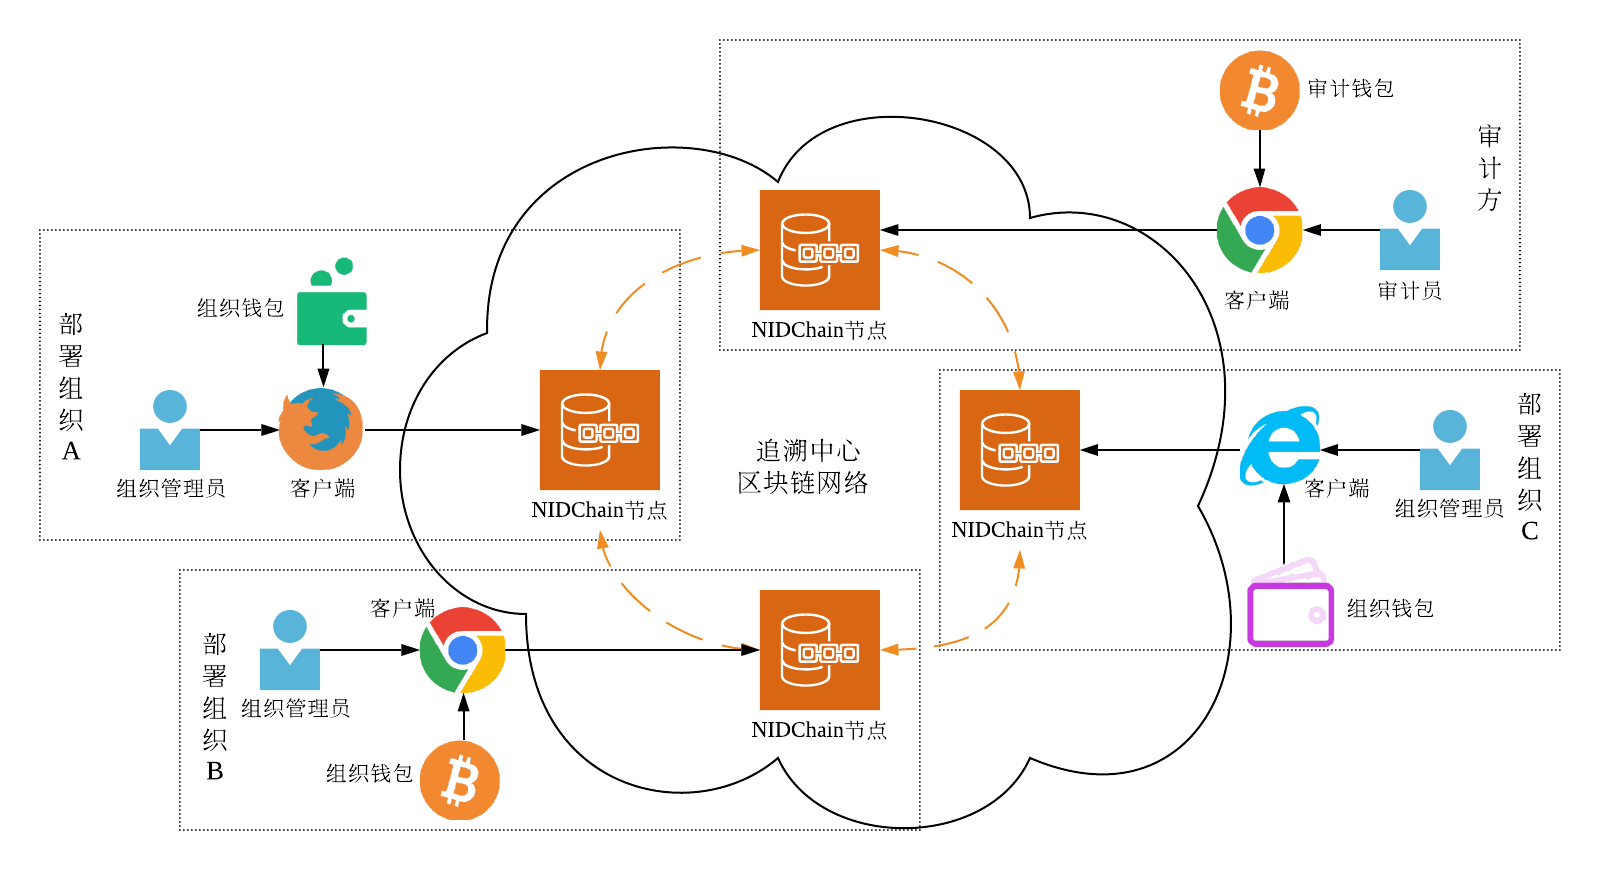
\includegraphics[width=\textwidth]{blockchain_nid_chain_architecture.png}
      \caption{NIDChain设计架构}
      \label{fig:blockchain_nid_chain_architecture}
    \end{figure}

    在建立NIDChain网络时,由审计方创建创世区块,并部署用于创建和维护组织信息的智能合约,本文将其命名为NIDAdmin。当有新的组织部署用户身份识别与溯源系统时,其启用一个新的区块链节点,连接进入NIDChain网络,同步区块链数据。组织管理员通过发布交易调用NIDAdmin,由NIDAdmin为该组织部署一个新的智能合约用于记录该组织的相关信息与密钥更新历史,本文将这类维护特定组织信息的智能合约命名为NIDOrg。

    本文设计NIDAdmin与NIDOrg中维护的信息分别如表\ref{tab:contract_NIDAdmin_information}与所示。其中OrgUpdateMsg为携带组织信息的结构体,其将在\ref{NIDTGA_Security:design:maintain}节中定义。KeyUpdateMsg为组织密钥更新消息的结构体,携带了组织历次密钥生成的密文与对应的生效时间,其设计为密文形式存储的原因将在\ref{NIDTGA_Security:design:authority}节说明。
    \begin{table}[htb]
      \centering
      \begin{minipage}[t]{\linewidth} 
        \caption{合约NIDAdmin信息列表}
        \label{tab:contract_NIDAdmin_information}
        \begin{tabularx}{\linewidth}{cc>{\centering\arraybackslash}X}
          \toprule[1.5pt]
          {\heiti 属性名} & {\heiti 类型} & {\heiti 说明} \\\midrule[1pt]
          public\_key & String & 审计方公钥 \\ 
          app\_queue & OrgUpdateMsg Array & 待审批的组织信息更新请求列表 \\ 
          org\_queue & NIDOrg Array & 记录组织信息的列表 \\
          \bottomrule[1.5pt]
        \end{tabularx}
      \end{minipage}
    \end{table}

    \begin{table}[htb]
      \centering
      \begin{minipage}[t]{\linewidth} 
        \caption{合约NIDOrg信息列表}
        \label{tab:contract_NIDOrg_information}
        \begin{tabularx}{\linewidth}{cc>{\centering\arraybackslash}X}
          \toprule[1.5pt]
          {\heiti 属性名} & {\heiti 类型} & {\heiti 说明} \\\midrule[1pt]
          org\_info & OrgUpdateMsg & 组织最新信息,包括组织名称、负责人联系方式、拥有的IPv6地址资源等 \\ 
          key\_history & KeyUpdateMsg Array & 组织密钥历史,以密钥密文与生效时间对的数组形式存储 \\ 
          \bottomrule[1.5pt]
        \end{tabularx}
      \end{minipage}
    \end{table}

    为了使与追溯功能相关的所有信息均记录在区块链上,以确保所有组织信息更新、密钥更新与用户追溯行为均可审计,因此本文将包括组织信息更新功能在内的所有能力,均通过智能合约NIDAdmin与NIDOrg提供给审计方或各个组织:
    \begin{enumerate}[1{)}]
      \item \textbf{组织信息更新}:组织信息更新实行由组织管理员提交申请、审计方进行批准的管理方式。组织管理员通过客户端连接区块链节点,使用本组织的私钥签发一条交易发布到NIDChain网络中,交易中包含对智能合约NIDAdmin的调用,完成申请的提交。审计方可通过区块链节点查看已有的申请,当需要批准或拒绝申请时,审计方使用自身私钥签发交易调用NIDAdmin的函数进行批准或拒绝。
      \item \textbf{组织密钥更新}:组织管理员使用客户端连接NIDChain节点,由客户端使用审计方的公钥将所要提交的新IDEA密钥加密后,与组织标识、密钥生效时间一起作为NIDOrg的输入,生成交易并使用本组织私钥签发后发布到NIDChain网络中。
      \item \textbf{用户身份追溯}:审计方连接区块链节点,调用NIDAdmin获取NIDTGA地址所属组织的密钥历史密文,审计方客户端利用私钥对密文进行解密,获取密钥明文历史,追溯获得用户NID,然后向用户组织的身份管理服务器查询用户真实身份。
    \end{enumerate}


    \subsection{追溯权限控制机制}
    \label{NIDTGA_Security:design:authority}
    数据公开透明是区块链的一个重要特点,由于每一个区块链节点都记录了完整的数据信息,因此写入区块链的任何数据对于区块链节点而言都是可见的。但是,对NIDTGA地址进行身份追溯的权限应该仅开放给审计方,避免不具有审计资格的人员能够根据NIDTGA地址追溯到其他组织内的用户身份,因此普通的组织管理员不应该能够获取得到其他组织的IDEA密钥明文历史。

    为了达成这个目的,在向区块链中写入组织更新的密钥时,必须对其进行加密,使得仅有审计方能够对密文进行解密。本文采用椭圆曲线算法\cite{koblitz1987elliptic,miller1985use}来解决这一问题,如图\ref{fig:NIDChain_key_update}所示。
    
    \begin{figure}[ht]
      \centering
      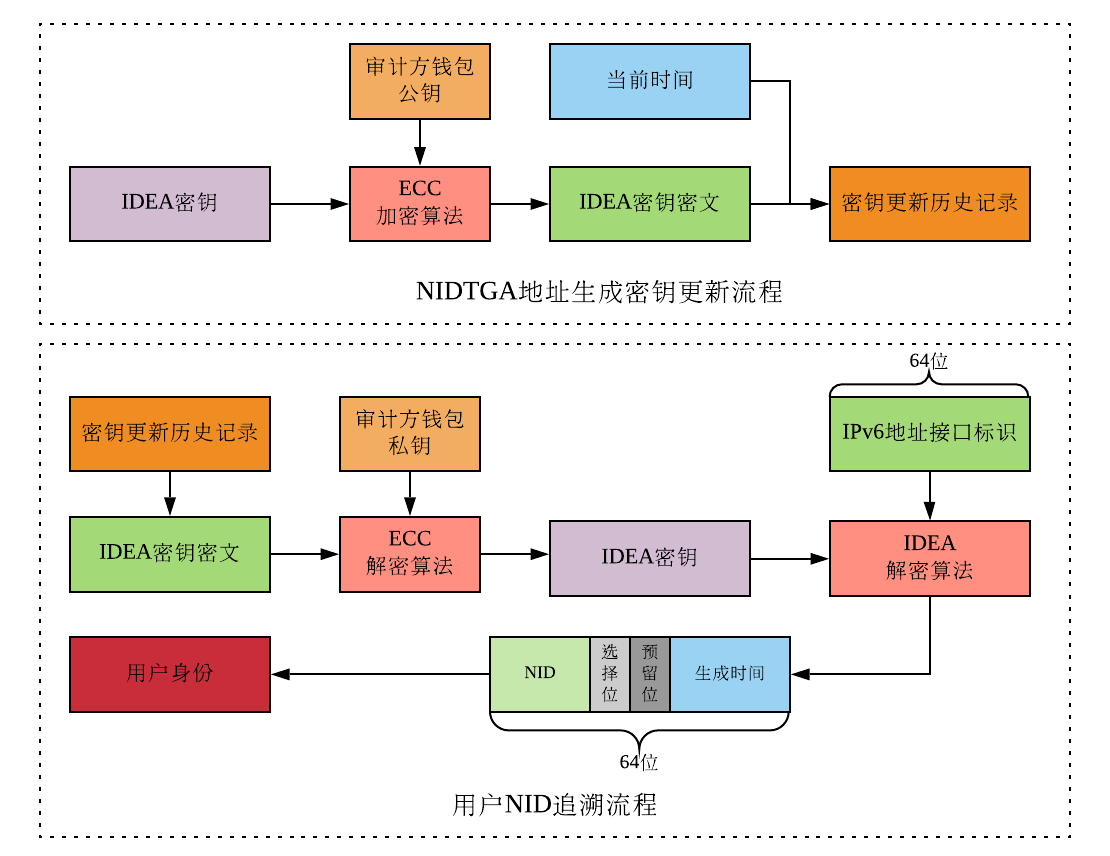
\includegraphics[width=\textwidth]{figures/NIDChain_key_update.png}
      \caption{NIDChain追溯权限控制机制示意}
      \label{fig:NIDChain_key_update}
    \end{figure}
    
    ECC算法使用的参数与区块链中钱包的公私钥对生成参数保持一致,以比特币采用的secp256k1\cite{qu1999sec}为例:
    \begin{enumerate}[1{)}]
      \item 组织管理员获取审计方公钥$public\_key$,采用secp256k1的参数设置对IDEA密钥$key$进行椭圆曲线加密,生成$encrypted\_key$。
      \item 审计方使用私钥$secret\_key$对$encrypted\_key$进行解密,获得明文$key$。其他组织的区块链节点虽然能够获得每个组织历次更新的$encrypted\_key$,但由于没有$secret\_key$,因而无法获得$key$。
    \end{enumerate}

    \subsection{组织信息更新机制}
    \label{NIDTGA_Security:design:maintain}
    组织信息更新发生在有新组织部署用户身份识别与溯源系统或已部署的组织变更其身份认证管理服务器信息与组织管理员等信息时,本文设计组织信息更新消息的结构如表\ref{tab:blockchain_design_organization_update_message}所示,将其命名为OrgUpdateMsg。
    \begin{table}[htb]
      \centering
      \begin{minipage}[t]{\linewidth} 
        \caption{组织信息更新消息OrgUpdateMsg格式}
        \label{tab:blockchain_design_organization_update_message}
        \begin{tabularx}{\linewidth}{cc>{\centering\arraybackslash}X>{\centering\arraybackslash}X}
          \toprule[1.5pt]
          {\heiti 属性名} & {\heiti 类型} & {\heiti 举例} & {\heiti 说明} \\\midrule[1pt]
          name & String & 张三 & 组织管理员姓名  \\ 
          phone & String & 13845678576 & 组织管理员电话 \\ 
          email & String & zs@tsinghua.edu.cn & 组织管理员邮箱 \\ 
          nid\_addr & String & 2402:f000:1:1011::1 & 组织用户身份管理服务器IPv6地址 \\ 
          port & Integer & 8888 & 供审计方通信的组织用户身份管理服务器传输层端口号 \\ 
          ipv6\_pool & String Array & [2402:f000:1:1001::, 2402:f000:1:1002::] & 组织用于生成NIDTGA地址的IPv6前缀列表 \\
          \bottomrule[1.5pt]
        \end{tabularx}
      \end{minipage}
    \end{table}

    组织在部署用户身份识别与溯源系统后,必须向NIDAdmin更新其组织信息。第一次更新组织信息被称为组织注册,NIDAdmin将以组织注册交易的发起地址作为唯一的组织标识,与记录该组织信息的NIDOrg合约相绑定,在后续组织信息更新时NIDAdmin将对其组织标识进行校验,要求更新组织信息的交易发起地址与对应的NIDOrg组织标识一致。OrgUpdateMsg中各属性在组织注册时必须提供合法的值,在后续的组织信息更新时可为空,NIDAdmin将认为其对应字段不修改。

    组织管理员填写组织信息更新消息后,经由客户端发起交易,调用智能合约NIDAdmin提供的组织信息更新函数,本文将其命名为orgUpdate。NIDChain收到该交易后进行共识,调用各自维护的NIDAdmin合约执行相关调用。orgUpdate操作执行成功后,组织的信息并未真正更新,而是被NIDAdmin添加到待审批列表app\_queue内。审计方将查看NIDAdmin的app\_queue,对组织的信息维护操作进行审批,通过调用NIDAdmin的updateApprove与updateReject函数分别批准或拒绝组织的信息维护,经过批准的组织信息将被更新到NIDAdmin内实际的组织列表org\_queue中。组织信息更新的时序如图\ref{fig:blockchain_organization_update_procedure}所示。

    \begin{figure}[ht]
      \centering
      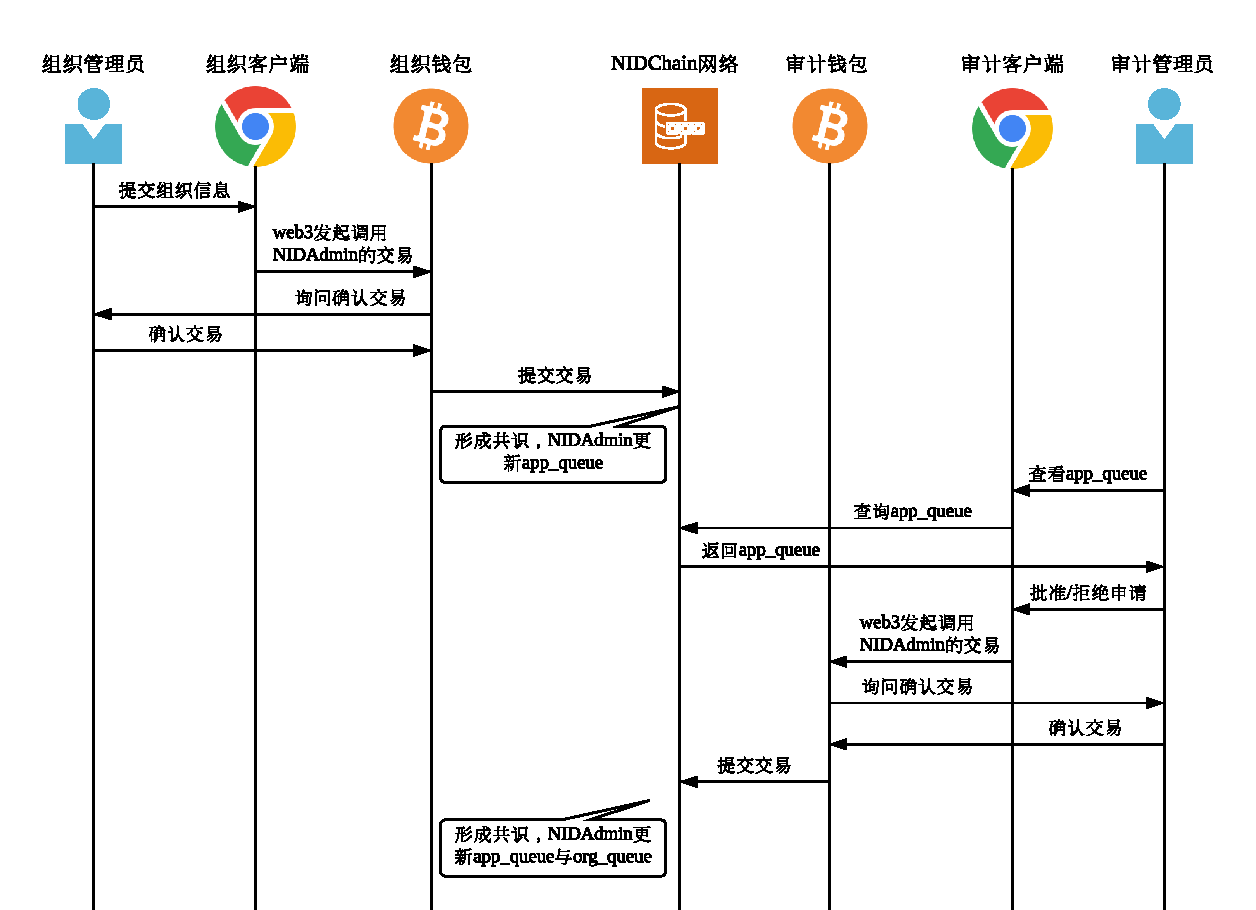
\includegraphics[width=0.9\textwidth]{blockchain_organization_update_procedure.pdf}
      \caption{NID组织信息更新时序}
      \label{fig:blockchain_organization_update_procedure}
    \end{figure}

    智能合约NIDAdmin中将维护app\_queue与org\_queue两个列表,其中app\_queue记录了各组织管理员已提交但待审批的组织信息,org\_queue中记录了目前已部署用户身份识别与溯源系统的各组织的信息。审计方可通过查看app\_queue审批组织信息的更新申请,被批准的组织信息将根据其组织标识更新org\_queue中对应组织的信息。org\_queue中每一个组织状态均由一个智能合约NIDOrg维护,当组织标识不在org\_queue的列表中时,说明该组织为新部署用户身份识别与溯源系统,NIDAdmin将为其创建一个新的NIDOrg合约并加入org\_queue中。

    NIDAdmin为组织信息更新机制提供的相关函数总结如表\ref{tab:contract_organization_update_function}所示。

    \begin{table}[htb]
      \centering
      \begin{minipage}[t]{\linewidth} 
        \caption{NIDAdmin组织信息更新相关函数}
        \label{tab:contract_organization_update_function}
        \begin{tabularx}{\linewidth}{cc>{\centering\arraybackslash}Xc>{\centering\arraybackslash}X}
          \toprule[1.5pt]
          {\heiti 函数名} & {\heiti 参数类型} & {\heiti 返回类型} & {\heiti 调用者} & {\heiti 说明} \\\midrule[1pt]
          orgUpdate & OrgUpdateMsg & 无 & 组织管理员 & 接收组织信息更新请求,加入待审核列表 \\ 
          updateQuery & 无 & OrgUpdateMsg Array & 审计方 & 查询待审批的组织信息更新请求列表 \\ 
          updateApprove & String & 无 & 审计方 & 接收组织钱包地址,通过相应组织信息更新请求 \\ 
          updateReject & String & 无 & 审计方 & 接收组织钱包地址,拒绝相应组织信息更新请求 \\ 
          \bottomrule[1.5pt]
        \end{tabularx}
      \end{minipage}
    \end{table}


    \subsection{组织密钥更新机制}
    \label{NIDTGA_Security:design:update}
    组织密钥更新发生在组织管理员更新用于NIDTGA地址接口标识加密的IDEA密钥时。用户身份识别与溯源系统在更新本地DHCPv6服务器的密钥前,需要由组织管理员先向NIDChain提交组织密钥更新,以确保在DHCPv6服务器使用新的密钥生成地址时,审计方已经可以使用新密钥对最新地址进行追溯。本文称组织客户端向NIDChain网络提交的组织密钥更新消息为KeyUpdateMsg,包含两个属性,一个是encrypted\_key,由组织管理员填写,用于携带经过ECC加密后的IDEA密钥密文,另一个是effect\_time,在发起交易时由程序按照当前时间自动填充,用于携带密钥更新时间,如表\ref{tab:blockchain_design_key_update_message}所示。之所以需要在密钥更新消息中由客户端主动填充当前时间,而不使用实际更新区块链数据时的时间作为密钥生效时间,是由于区块链的数据更新对客户端而言是一个异步操作,其需要等待交易被打包进新的区块,并等待新区块在区块链网络中形成共识,在区块链运行智能合约的虚拟机内部难以获知现实时间的确切时间,其仅能通过区块的共识时间了解当前所处的时间区间,因此如果采用区块时间作为新密钥的生效时间,将导致记录的生效时间比实际生效时间严重滞后。

    \begin{table}[htb]
      \centering
      \begin{minipage}[t]{\linewidth} 
        \caption{组织密钥更新消息KeyUpdateMsg格式}
        \label{tab:blockchain_design_key_update_message}
        \begin{tabularx}{\linewidth}{cc>{\centering\arraybackslash}X>{\centering\arraybackslash}X}
          \toprule[1.5pt]
          {\heiti 名称} & {\heiti 类型} & {\heiti 举例} & {\heiti 说明} \\\midrule[1pt]
          encrypted\_key & String & b/zHpAdf+W1PgGW Wcw+LqBrvJ1lVhO nsIOzd+BkVi1JII Trionfx+gM90TaV 0uxDY6mqBgsN3z kXcyaMYRizOA== & IDEA密钥经过审计方公钥使用ECC加密后的密文 \\ 
          effect\_time & Integer & 1586916525 & 密钥生效时间 \\ 
          \bottomrule[1.5pt]
        \end{tabularx}
      \end{minipage}
    \end{table}

    当组织管理员通过客户端更新IDEA密钥时,客户端首先向NIDChain查询获取审计方公钥,通过ECC加密算法将新的IDEA密钥进行加密,形成KeyUpdateMsg后,签发交易调用智能合约NIDOrg提供的密钥更新函数keyUpdate,将新的密钥追加至其密钥历史key\_history的队尾。key\_history中每一条记录均记录了每次更新的密钥密文与生效时间。执行成功后,客户端再将IDEA密钥的明文通过TLS发送给本地的DHCPv6服务器进行更新。

    组织密钥更新机制中涉及的智能合约函数总结如表\ref{tab:contract_key_update_function}所示。
    \begin{table}[htb]
      \centering
      \begin{minipage}[t]{\linewidth} 
        \caption{NIDOrg组织密钥更新相关函数}
        \label{tab:contract_key_update_function}
        \begin{tabularx}{\linewidth}{c>{\centering\arraybackslash}Xcc>{\centering\arraybackslash}X}
          \toprule[1.5pt]
          {\heiti 函数名} & {\heiti 参数类型} & {\heiti 返回类型} & {\heiti 调用者} & {\heiti 说明} \\\midrule[1pt]
          keyUpdate & KeyUpdateMsg & 无 & 组织管理员 & 更新对应组织密钥历史 \\
          \bottomrule[1.5pt]
        \end{tabularx}
      \end{minipage}
    \end{table}
    
    \subsection{用户身份追溯机制}
    \label{NIDTGA_Security:design:trace}
    用户身份追溯由审计方发起,需要经历图\ref{fig:blockchain_nid_trace_procedure}所示过程:
    \begin{enumerate}[1{)}]
      \item \textbf{查询组织密钥历史}:审计方通过客户端以NIDTGA地址作为参数调用合约NIDAdmin,NIDAdmin根据NIDTGA地址的前缀,查询NIDOrg列表,确定其所属组织,将该组织的信息与密钥历史返回客户端。客户端使用审计方私钥,从组织密钥历史队尾开始逐个向前解密获得IDEA密钥明文,用于尝试解密NIDTGA地址的接口标识,获得用户NID与上网时间。
      \item \textbf{查询用户真实身份}:审计方将用户真实身份查询请求用私钥采用ECC算法签名后发送给该组织用户身份管理服务器,与用户身份管理服务器的通信信息由NIDOrg中的nid\_addr与port确定。用户身份管理服务器使用审计方公钥对数字签名进行验证后,答复NID对应用户的真实身份,答复同样将用户真实身份使用审计方公钥加密,以防止被攻击者窃听获取。
    \end{enumerate}

    \begin{figure}[ht]
      \centering
      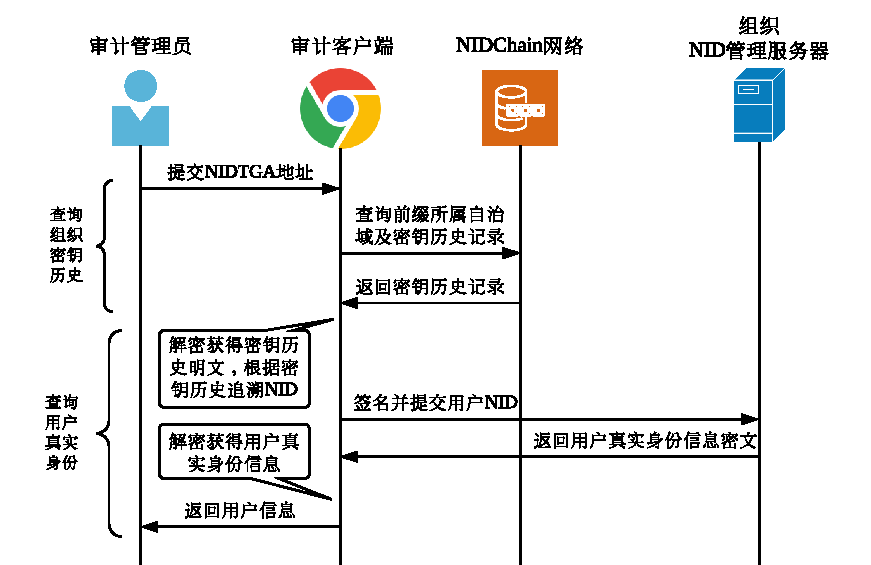
\includegraphics[width=\textwidth]{blockchain_nid_trace_procedure.pdf}
      \caption{NIDChain用户真实身份追溯时序}
      \label{fig:blockchain_nid_trace_procedure}
    \end{figure}

    因此,本文设计NIDAdmin与NIDOrg提供用户组织查询的函数如表\ref{tab:contract_org_query_function}所示。
    \begin{table}[htb]
      \centering
      \begin{minipage}[t]{\linewidth} 
        \caption{用户组织查询相关函数}
        \label{tab:contract_org_query_function}
        \begin{tabularx}{\linewidth}{ccccc>{\centering\arraybackslash}X}
          \toprule[1.5pt]
          {\heiti 合约名} & {\heiti 函数名} & {\heiti 参数类型} & {\heiti 返回类型} & {\heiti 调用者} & {\heiti 说明} \\\midrule[1pt]
          NIDAdmin & orgQuery & String & NIDOrg & 审计方 & 接受NIDTGA地址作为参数,返回该地址所属组织的信息 \\ 
          NIDOrg & addrCheck & String & Boolean & NIDAdmin & 判断NIDTGA地址是否属于该组织,是则返回True \\ 
          \bottomrule[1.5pt]
        \end{tabularx}
      \end{minipage}
    \end{table}

    由于客户端在更新密钥时,由客户端填充密钥更新消息中的密钥生效时间,而后再更新本地生成NIDTGA地址的密钥,因此区块链中记录的密钥生效时间将一定程度早于密钥的实际生效时间,如图\ref{fig:key_valid_time_drift}中DELTA所示。DELTA包含的时间主要由两部分组成:客户端向DHCPv6服务器传输新密钥的时间和在将新密钥更新至DHCPv6服务器内存中的时间。前者需要建立TLS的加密信道进行传输,后者需要获取保护加密密钥的读写锁以对内存中的密钥进行写入。在NIDTGA地址生成方案中,网络接口标识内嵌入的时间信息至多使用24位,以较为通用的Epoch时间计时,则至多支持2分钟为区分粒度。尽管DELTA在一般情况下远小于2分钟,但在网络拥塞导致密钥传输时间过长、DHCPv6服务器并发数过大导致读写锁迟迟未得到释放、密钥更新等待较久等极端情况下仍可能出现区块链中记录的时间信息与密钥实际生效时间属于不同粒度区间的情形,如图\ref{fig:key_valid_time_drift}中密钥0更新至密钥1时的红字所示。倘若某一NIDTGA地址恰好在新密钥生效所属的时间粒度区间内由旧密钥加密生成,则可能在追溯过程中校验时间信息时发生错误从而导致追溯失败。尽管这种情况发生的概率极低,但在客户端对组织密钥历史进行解密后,使用IDEA密钥明文解密NIDTGA地址的接口标识时,仍需要对密钥有效时间进行一定偏移拓展。因此,本文设计用户NID追溯过程如算法\ref{algo:blockchain_nid_trace}所示,对每个密钥的过期时间向后拓展1个NIDTGA地址中时间信息的粒度,但其生效时间仍按NIDChain中记录的生效时间为准。

    \begin{figure}[ht]
      \centering
      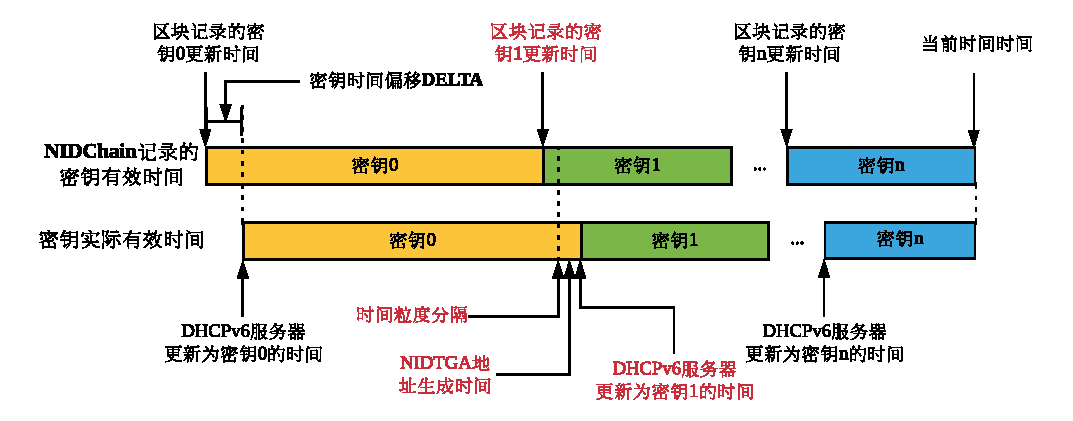
\includegraphics[width=\textwidth]{key_valid_time_drift.pdf}
      \caption{密钥记录时间与生效时间偏移示意}
      \label{fig:key_valid_time_drift}
    \end{figure}

    \begin{algorithm}
      \caption{用户NID追溯算法}
      \label{algo:blockchain_nid_trace}
      
      \LinesNumbered
      \SetKw{KwInList}{in}
      \SetKw{KwBreak}{break}
      \SetKw{KwTrue}{true}
      \SetKw{KwFalse}{false}
      \SetKw{KwAnd}{and}
      \SetKw{KwDownto}{downto}
      \SetKw{KwReturn}{return}
      \SetKw{KwAssert}{assert}
      \KwIn{NIDTGA\_address, key\_time\_array}
      \KwOut{NID}

      expired\_time \gets getEpochTime()\;
      n \gets key\_time\_array.length()\;
      \For{i = n - 1 \KwDownto 0}{
        key \gets key\_time\_array.getKey()\;
        effect\_time \gets key\_time\_array.getTime()\;
        decrypted\_interface \gets decryptInterface(NIDTGA\_address, key)\;
        interface\_time \gets parseTimeFromInterface(decrypted\_interface)\;
        \If{interface\_time > effect\_time \KwAnd interface\_time < expired\_time} {
          \KwReturn parseNIDFromInterface(decrypted\_interface)\;
        }
        expired\_time \gets effect\_time + NIDTGA\_TIME\_INTERVAL\;  
      }
      \KwAssert(\KwFalse);
    \end{algorithm}


    获得用户NID的追溯后,审计方客户端将向对应组织的用户身份管理服务器查询用户的真实身份。审计方客户端与用户身份管理服务器通信时的请求与答复消息格式分别定义如表\ref{tab:blockchain_design_user_identity_request}与表\ref{tab:blockchain_design_user_identity_response}所示。其中答复消息中包含的encrypted\_other项采用JSON\cite{RFC7159}组织其他携带的信息,以实现更好的扩展性。
    \begin{table}[htb]
      \centering
      \begin{minipage}[t]{\linewidth} 
        \caption{用户真实身份请求消息格式}
        \label{tab:blockchain_design_user_identity_request}
        \begin{tabularx}{\linewidth}{cc>{\centering\arraybackslash}X>{\centering\arraybackslash}X}
          \toprule[1.5pt]
          {\heiti 名称} & {\heiti 类型} & {\heiti 举例} & {\heiti 说明} \\\midrule[1pt]
          nid & String & 80002888b1 & 所要查询身份的用户NID \\ 
          sign & String & MEYCIQDyVawkmvzi9YUXsWQF Hr4os0B4oSuwynf5DxBLsUb8iwIh APIcnbL2id/SLoxdsNhRKgsuCYZs S5bGsoWjxgny2geU & 审计方私钥对NID的签名 \\ 
          \bottomrule[1.5pt]
        \end{tabularx}
      \end{minipage}
    \end{table}

    \begin{table}[htb]
      \centering
      \begin{minipage}[t]{\linewidth} 
        \caption{用户真实身份答复消息格式}
        \label{tab:blockchain_design_user_identity_response}
        \begin{tabularx}{\linewidth}{cc>{\centering\arraybackslash}X>{\centering\arraybackslash}X}
          \toprule[1.5pt]
          {\heiti 名称} & {\heiti 类型} & {\heiti 举例} & {\heiti 说明} \\\midrule[1pt]
          encrypted\_name & String & kEZdlv+2AT0V8PVq FCkOdSLG3w3Z5reB 7ZfDHfxR1rSLT90K yrxsSP8= & NID对应用户姓名用审计方公钥加密后的结果 \\ 
          encrypted\_other & String & LFJjCGyhUxHnWdJu QdYdDEFmDoSMLMy+ 5/a0/KPzQlTQGCqE UxcHq09HStSZ & 用户其他信息以JSON格式表示后用审计方公钥加密后的结果 \\ 
          \bottomrule[1.5pt]
        \end{tabularx}
      \end{minipage}
    \end{table}


  \section{基于以太坊的用户身份溯源系统实现}
  \label{NIDTGA_Security:implement}
  采用区块链实现的用户身份溯源系统的一个潜在问题是,由于存在所有区块链节点之间的共识过程,其所有信息的写入均不是实时的,需要等待下一个区块的产生,尽管我们可以通过调整PoW算法的难度值来提升其出块速度,但其仍与即时写入的单点数据库性能有所差距。考虑到各组织信息更新与用户追溯操作并不频繁且实时性要求并不高,本文仍采用以太坊作为用户身份溯源系统的实现平台,以达到更强的安全性。NIDChain的以太坊应用架构与RegChain类似,开发使用的技术栈也相同,在此不再赘述。项目代码参见NIDChain的Git仓库\footnote{NIDChain repository, https://github.com/BragCat/NIDChain}。

    \subsection{DApp}
    \label{NIDTGA_Security:implement:DApp}
  
    在NIDChain中,要实现的DApp主要包含NIDAdmin与NIDOrg两个智能合约。两者需要维护的内部状态已由表\ref{tab:contract_NIDAdmin_information}与表\ref{tab:contract_NIDOrg_information}分别定义,在使用Solidity对其进行实现时,分别采用如表\ref{tab:ethereum_NIDAdmin_attributes}与表\ref{tab:ethereum_NIDOrg_attributes}的数据结构。其中OrgInfo结构体与OrgUpdateMsg消息格式一致,各属性类型均有Solidity对应的内置类型,在此不再赘述。KeyTime结构体即为包含了string类型的$encrypted\_key$与uint256类型的$time$两个属性的密钥历史。
    \begin{table}[htb]
      \centering
      \begin{minipage}[t]{\linewidth} 
        \caption{合约NIDAdmin数据结构}
        \label{tab:ethereum_NIDAdmin_attributes}
        \begin{tabularx}{\linewidth}{ccc>{\centering\arraybackslash}X}
          \toprule[1.5pt]
          {\heiti 属性名} & {\heiti 类型} & {\heiti Solidity数据结构} & {\heiti 说明} \\\midrule[1pt]
          public\_key & String & string & 审计方公钥,在部署合约时由部署者的公钥初始化 \\ 
          app\_queue & OrgUpdateMsg Array & mapping(bytes20 => OrgInfo) & 待审批的组织信息更新请求哈希映射表,以组织地址为索引,组织更新请求OrgInfo为值 \\ 
          org\_queue & NIDOrg Array & mapping(bytes20 => NIDOrg) & 组织哈希映射表,以组织地址为索引,组织合约NIDOrg为值 \\
          \bottomrule[1.5pt]
        \end{tabularx}
      \end{minipage}
    \end{table}

    \begin{table}[htb]
      \centering
      \begin{minipage}[t]{\linewidth} 
        \caption{合约NIDOrg数据结构}
        \label{tab:ethereum_NIDOrg_attributes}
        \begin{tabularx}{\linewidth}{ccc>{\centering\arraybackslash}X}
          \toprule[1.5pt]
          {\heiti 属性名} & {\heiti 类型} & {\heiti Solidity数据结构} & {\heiti 说明} \\\midrule[1pt]
          org\_info & OrgUpdateMsg & OrgInfo & 组织最新信息 \\ 
          key\_history & KeyTimePair Array & KeyTime[] & 组织密钥历史,按时间顺序进行记录历次更新密钥与时间,队尾最新 \\ 
          \bottomrule[1.5pt]
        \end{tabularx}
      \end{minipage}
    \end{table}

    对于NIDAdmin中的两个队列,本文采用了哈希映射表而非数组的形式,以更好地支持根据组织标识查找组织相关信息。NIDAdmin与NIDOrg分别实现了\ref{NIDTGA_Security:design}节中提到的各个函数,并且采用了modifier对各函数调用者身份进行了限定,比如采用openzeppelin\footnote{Openzeppelin,https://docs.openzeppelin.com/openzeppelin/}中提供的onlyOwner将NIDAdmin.orgQuery的调用方限制为审计方等。

    \subsection{客户端}
    \label{NIDTGA_Security:implement:client}
    NIDChain的客户端与RegChain不同,不需要与类似于ACS服务器软件的程序进行互操作,仅面向组织管理员与审计人员提供服务,因此客户端采用完全基于React的网页应用。其各个页面与RegChain中所示类似,在此不再反复展示。

    客户端通过Web3.js使用JSON RPC的格式与区块链节点进行交互,其针对组织管理员与审计方分别实现了如表\ref{tab:nid_org_client_callback_function}和表\ref{tab:nid_trace_client_callback_function}所列的回调函数。
    \begin{table}
      \centering
      \begin{minipage}[t]{\linewidth} 
        \caption{用户身份溯源系统以太坊实现的组织客户端回调函数}
        \label{tab:nid_org_client_callback_function}
        \begin{tabularx}{\linewidth}{ccc>{\centering\arraybackslash}X}
          \toprule[1.5pt]
          {\heiti 函数名} & {\heiti 参数名} & {\heiti 参数类型} & {\heiti 说明} \\\midrule[1pt]
          handleOrgUpdate & org\_info & OrgInfo &组织管理员填写组织信息表单并点击提交按钮后,将组织信息组织成JSON格式发起调用NIDAdmin.orgUpdate函数的交易 \\ 
          handleKeyUpdate & key & string & 组织管理员填写新密钥并点击提交按钮后,向区块链查询得审计方公钥并将key加密,发起调用NIDOrg.keyUpdate函数的交易 \\
          \bottomrule[1.5pt]
        \end{tabularx}
      \end{minipage}
    \end{table}

    \begin{table}
      \centering
      \begin{minipage}[t]{\linewidth} 
        \caption{用户身份溯源系统以太坊实现的审计方客户端回调函数}
        \label{tab:nid_trace_client_callback_function}
        \begin{tabularx}{\linewidth}{ccc>{\centering\arraybackslash}X}
          \toprule[1.5pt]
          {\heiti 函数名} & {\heiti 参数名} & {\heiti 参数类型} & {\heiti 说明} \\\midrule[1pt]
          handleGetUpdateApply & 无 & 无 & 审计方点击查询按钮后,向区块链查询获得目前待审批的组织信息更新请求 \\ 
          handleUpdateApprove & id & string & 审计方点击某一请求的通过按钮后,以该组织标识发起调用NIDAdmin.updateApprove函数的交易 \\ 
          handleUpdateReject & id & string &  审计方点击某一请求的拒绝按钮后,以该组织标识发起调用NIDAdmin.updateReject函数的交易 \\ 
          handleUserQuery & nidtga & string & 审计方填写待追溯的NIDTGA地址并点击查询按钮后,首先调用NIDAdmin.orgQuery函数获得用户所属组织信息,然后用审计方私钥对其密钥历史进行解密,根据密钥历史解密NIDTGA地址的接口标识获得用户NID,将NID用私钥签名后发送给组织用户身份管理服务器获得用户真实身份 \\
          \bottomrule[1.5pt]
        \end{tabularx}
      \end{minipage}
    \end{table}

    \subsection{系统测试与讨论}
    \label{NIDTGA_Security:implement:test}

      \subsubsection{性能测试}
      \label{NIDTGA_Security:implement:test:performance}
      NIDChain支持的各项操作均由客户端侧与DApp侧两部分组成。对于客户端侧的操作,组织信息维护、更新审批均只需要签发交易,开销应较小,而组织密钥更新与用户身份追溯则涉及到ECC加解密的过程,耗时应该较多。区块链侧操作主要是等待交易打包出块、执行智能合约,因此耗时与区块链出块速度、智能合约执行速度有关。以太坊的出块速度与创建创世区块时的难度值相关,而与网络规模不相关,为提升其共识速度可以将难度值设定为一个较小值。但由于NIDChain中并不会频繁发生更新数据的交易,因此过高的出块速度将导致区块链中包含大量空的区块,使区块链过于臃肿。因此,本文在测试时将创世区块的难度值设定为0x4cccc8,平均15秒左右生成一个区块,一方面使得客户可以比较快地看到自己提交的数据被写入区块链,另一方面也不会造成区块链存储资源的过度浪费。

      为了较为真实地模拟NIDChain的实际运行环境,本文以CNGI-CERNET2接入41所高校为例,采用41个区块链节点的网络规模对用户身份溯源系统的各项功能的性能进行了测试,结果如表\ref{tab:nid_ethereum_performance}所示。
      \begin{table}[htb]
        \centering
        \begin{minipage}[t]{\linewidth} 
          \caption{用户身份溯源系统的以太坊实现性能测试}
          \label{tab:nid_ethereum_performance}
          \begin{tabularx}{\linewidth}{>{\centering\arraybackslash}X>{\centering\arraybackslash}X>{\centering\arraybackslash}X}
            \toprule[1.5pt]
            {\heiti 功能} & {\heiti 客户端时间(ms)} & {\heiti 合约时间(ms)} \\\midrule[1pt]
            {\heiti 组织信息维护} & 7 & 136 \\ 
            {\heiti 组织密钥更新} & 69 & 78 \\ 
            {\heiti 组织信息更新通过} & 6 & 152 \\ 
            {\heiti 组织信息更新拒绝} & 6 & 160 \\ 
            {\heiti 用户身份追溯} & 132 & 69 \\ 
            \bottomrule[1.5pt]
          \end{tabularx}
        \end{minipage}
      \end{table}

      可见,组织信息维护、更新通过与拒绝等操作的客户端耗时极少,而组织密钥更新与用户身份追溯操作在客户端侧的耗时较多,与分析一致。而在DApp侧,组织信息维护、更新审批操作由于需要维护NIDAdmin内部队列,因此耗时较组织密钥更新操作更多,而用户身份追溯只需要读取NIDChain的数据而不需要更改合约状态,因此耗时最短。总而言之,对客户而言,其在客户端进行NIDChain所支持的各项操作耗时均不足1秒,提交的数据被写入区块链至多等待15秒即可被出块并进行查询,具有良好的性能。

      \subsubsection{安全性讨论}
      \label{NIDTGA_Security:implement:test:security}
      用户身份溯源系统的以太坊实现包含以下几个方面的安全性:
      \begin{enumerate}[1{)}]
        \item \textbf{密钥安全}:密钥历史安全指的是写入区块链的密钥历史不会被恶意篡改或被非授权用户读取。防止恶意篡改的机制由以太坊的共识算法提供,本文在测试时手动更改了NIDChain中1至20个节点的数据,实验证明在不更改网络中大部分节点数据的情况下,非恶意的区块链节点将校验并承认获得最多节点共识的数据,通过客户端请求时可以获得未遭篡改的数据。防止非授权用户读取密钥的机制由本文设计的采用审计方公钥进行ECC加密的机制保证,对于NIDChain中的每个节点,其只能获取得到历次组织密钥加密后的密文,在不拥有审计方私钥的前提下无法对其进行解密获得密钥原文。
        \item \textbf{服务安全}:服务安全指的是在NIDChain中若干节点遭受攻击而宕机或服务不可用时,其仍能够向审计方和组织方提供追溯或信息更新服务。本文在对NIDChain的测试中,将节点数从41逐渐减至1,在自身组织的区块链节点可达的情况下,客户端仍可以其作为web3.js的provider连接NIDChain进行操作,说明在NIDChain中至少还有一个节点存活的情况下,服务可用性始终可以得到保障。
        \item \textbf{合约安全}:合约安全是指智能合约本身不存在可供利用的安全漏洞,常见的安全漏洞有:未加保护的函数调用、交易依赖攻击、类型溢出攻击等。本文的实现中对每个函数调用均采用了modifier修饰以确保仅有合约的合法拥有者可以调用合约的各个函数,在每个函数的内部增加了参数范围检查,以避免类型溢出攻击。
      \end{enumerate}

      总而言之,NIDChain在密钥安全与服务安全方面对用户身份识别与溯源系统中全局唯一的追溯服务器设计进行了改进,避免了数据篡改与拒绝服务攻击的问题,同时也没有引入明显的新安全问题,显著提升了用户身份识别与溯源系统的安全性。

  \section{本章小结}
  \label{NIDTGA_Security:summary}
  本章从用户身份识别与溯源系统的安全性出发,分析了系统在多个管理域内得到部署推广的情形下,用户接入与身份溯源各环节的安全性保障,对其追溯功能设计的安全隐患进行了探讨,并提出使用区块链构建用户身份溯源系统NIDChain,以保证各组织信息、密钥历史的数据安全与追溯功能的高可用。本章给出了NIDChain的详细设计,并采用以太坊对其进行了实现与测试,证明了NIDChain的可行性,有效提升了用户身份识别与溯源系统在多组织部署时的安全性。
